
% # Preamble

% ## Doc Class
\documentclass{beamer}

% ## Pkgs
\usepackage{perpage} % makes foonotes per page with a commmand
\usepackage{graphicx}
\usepackage{booktabs}
\usepackage{amsmath}
\usepackage{dcolumn}
\usepackage{caption}
\usepackage{tikz}

% ## Theme
\usetheme{Madrid}

% ## Having Presentation Notes

% \setbeameroption{show notes on second screen} % comment out this line to get without notes version for the purpose of distribution
% \setbeameroption{show notes} % note pages are interleaved with slides
% \setbeameroption{hide notes}

% ## Other Settings

% \MakePerPage{footnote} % pkg: perpage, makes footnotes per page

\graphicspath{{./imgs/}} % pkg: graphicx, direcoty of images

\DeclareMathOperator{\E}{\mathbb{E}} % pkg: amsmath

% \newcolumntype{d}[1]{D{.}{.}{#1}} % pkg: dcolumn

% \setbeamertemplate{caption}[numbered] % make table and figs numbered
\setbeamertemplate{frametitle}[default][center]

% \usepackage{floatrow}
% \floatsetup[table]{font=rm}

% ## Title & Author

\title[]{\MakeUppercase{The Trading Behavior of Institutional and Individual Investors, Evidence from Iran}}
\subtitle{}

\author[]{Mahdi Mir \newline Supervised by: Dr. Mahdi Heidari}

\institute[]{TeIAS}

\date[]{}

% # Doc
\begin{document}


\begin{frame}
    \titlepage{}
\end{frame}

\begin{frame}[label=toc]
    \frametitle{Outline}
    \tableofcontents{}
\end{frame}


\section{Overview}
\subsection{Introduction}


\begin{frame}{Introduction}
    \begin{block}{Trading Strategy (Behavior) Litretature}
        \begin{itemize}
            \item This literature investigates about how different players in the financial markets react to recent price changes or returns. (The effect of price changes on investors behavior)
            \item Mostly, the literature investigates the existense and the strength of momentum or contrarian strategies among investors.(Griffin et al. (2003))
            \item These studies are categorized as a part of \textit{\textbf{Behavioral Finance}}.
        \end{itemize}
    \end{block}
\end{frame}

\begin{frame}{Introduction (cont'd)}
    \begin{block}{What Are The Momentum And Contrarian Strategies?}
        \begin{itemize}
            \item A momentum investor buys winners and sell losers, in contrast, a contrarian investor sells winners and buys losers.
            \item A momentum investor follows the trend and a contrarian does the opossite.
            \item Momentum strategy is also called \textbf{"Trend-Chasing"} or \textbf{"Positive Feedback Trading"}.
            \item Contrarian strategy is also called \textbf{"Anti-Momentum"}.
        \end{itemize}
    \end{block}
\end{frame}


\subsection{The Question, Expectations, Results Summary}


\begin{frame}{The Question}
    \begin{itemize}
        \item I am investigating the trading patterns of both Institutional and Individual investors in the Tehran Stock Exchange market.
        \item Specifically, I am asking whether these institutions and individuals tend to follow momentum or contrarian strategies when they trade.
        \item Also, do theoretical and empirical results of the literature hold in TSE?
        \item The focus is on institutions because they're major players in the market, and naturally we expect them to make trades based on fundamentals.
        \item I am exploring momentum and contrarian strategies because of how they can influence market herding. This might push prices far from their real values and even lead to market bubbles (Delong et al. (1990), Hong \& Stein(1999)).
    \end{itemize}
\end{frame}

\begin{frame}{Expectations}
    \begin{enumerate}
        \item Based on the extant literature (both theory and empirical), in general, institutional investors perform a momentum-trading strategy, individual investors perform an anti-momentum or contrarian trading strategy (Koesrindartoto et al.(2020)).
        \item We expect institutions to have a stronger herding behavior compared to individuals (Lakonishok, Shleifer, Vishny (1992)).
        \item As instutions are more focused on large firms we expect more stronger behavior from them in large firms comparing to small firms.
    \end{enumerate}
\end{frame}

\begin{frame}{Results Summary}
    \begin{block}{Results vs Expectations}
        \begin{itemize}
            \item Institutional investors follow momentum strategy in one week and one month periods. Individuals are contrarian in one month and three months periods. This aligns with the first expectation.
            \item Just like our second expectation, institutions herd more comparing to individuals.
            \item Confirming the third expectation, institutions have stronger behavior in large firms versus small firms.
        \end{itemize}
    \end{block}
\end{frame}


\subsection{Data}


\begin{frame}{Data}
    \begin{enumerate}
        \item \textbf{TSE Stocks' Retruns}, \textit{Daily}
        \item \textbf{TSE Overall Index Returns (Market Return)}, \textit{Daily}
        \item \textbf{CBI Risk-Free Rate}, \textit{Monthly}
        \item \textbf{All Codal News (Letters)}, \textit{Secondly}
              \begin{itemize}
                  \item Both before 1389 (1382 to 1389) and after 1389
              \end{itemize}
        \item \textbf{TSE Individual-Institutional Trade}, \textit{Daily}
        \item \textbf{TSE Stocks' Market Capitalization}, \textit{Daily}
        \item \textbf{TSE Stocks' Nominal Prices}, \textit{Daily}
    \end{enumerate}
\end{frame}


\section{Litretature Review}


\begin{frame}{Litretature Review}
    \begin{itemize}
        \item The literature on the trading behavior of investors is vast and diverse.
        \item Theoretically, institutional investors are viewed as informed investors with the power to drive the market, while individual investors are seen as proverbial noise traders with a tendency to engage in psychologically biased trading (Kyle (1985); Black (1985)).
    \end{itemize}
\end{frame}

\begin{frame}{Litretature Review (cont'd)}
    Why we expect institutions herdi more than individuals?
    \begin{enumerate}
        \item The institution will try to infer information about the quality of investment from one institution or another. As a result, institutions will have a greater understanding of each other’s trading practices than do individuals, and so will herd to a greater extent (Lakonishok et al. (1992); Shiller and Pound (1989); Banerjee (1992)).
        \item Second, institutional investors have an incentive to hold the same stocks as other money managers to avoid falling behind in peer group performance (Scharfstein and Stein (1990)).
        \item Third, an institution might react to the same exogenous signal, and since the signal received by institutions is typically the same, institutions tend to herd more than do individual investors.
    \end{enumerate}
\end{frame}

\begin{frame}{Litretature Review (cont'd)}
    \begin{itemize}
        \item Lakonishok et al. (1992) find weak evidence of herding behavior among pension funds managers using quarterly data of the NYSE.
        \item Ng, Wu (2007),Chinese institutions are momentum investors, while less wealthy Chinese individual investors at large are contrarian investors.
        \item Kaniel et al. (2008), on the other hand, take a different perspective and also find that individual investors are contrarian toward institutional investors. This contrarian tendency leads them to act as liquidity providers for institutional investors requiring immediate action.
        \item Koesrindartoto et al. (2020), using \(250 M\) transaction observations in Indonesia find that institutional investors are momentum traders and individual investors are contrarian traders in the Indonesian Stock Exchange.
    \end{itemize}
\end{frame}



\section{Methodology}


\begin{frame}{Methodology}
    This research has two stages:
    \begin{enumerate}
        \item The first stage revolves around the categorization of company-specific news as either positive or negative.
        \item In stage two, I analyze the trading behavior of institutions and individuals within mutally non-overlapping time frames.
    \end{enumerate}
\end{frame}


\subsection{Stage 1: News Labeling}


\begin{frame}
    \Huge
    \center
    Stage 1
    \\
    News Labeling
\end{frame}

\begin{frame}{Why News Are Important?}
    \begin{itemize}
        \item Abundant evidence suggests that news pertaining to individual stocks, characterized as either "positive" or "negative," significantly impacts the trading choices made by investors (Chan(2003), Chen-Hui \& Chan-Jane(2017)).
        \item Any study or research design intending to analyze the trading behavior of investors of any type must take into account information related to companies.
        \item Regrettably, we currently lack a database containing company-specific news curated through assessments and opinions from expert capital market analysts.
        \item Creating such a dataset would significantly enhance the research landscape within the Tehran Stock Exchange market.
    \end{itemize}
\end{frame}

\begin{frame}{How I Solve The News Challenge?}
    \begin{itemize}
        \item In the first stage, I use a syatematic and simple method for categorizing stock-specific news as either "Positive" or "Negative" or "Neutral".
        \item The labels generated during this initial stage are then employed in the second stage as dummy variables to account for the presence of "positive" and "negative" news associated with each individual stock.
    \end{itemize}
\end{frame}

\begin{frame}{How I Lebel News as Good or Bad?}
    To categorize news systematically:
    \begin{enumerate}
        \item I consider a two month window for each stock prior to each day.
        \item Within this moving window, I fit the CAPM model (Rolling CAPM approach).
        \item By utilizing the CAPM betas, I compute the expected return for each specific firm-day.
        \item Based on the calculated expected return in the previous step, I find the Abnormal Returns.
        \item Employing a symmetric threshold, I determine how news should be classified.
    \end{enumerate}
\end{frame}

\begin{frame}{Source of Firm-Specific News}
    \begin{itemize}
        \item I rely on Codal.ir for firm-specific news.
        \item I perceive every letter posted on Codal as a news item.
        \item Thankfully, each company-specific update on Codal is consistently linked to the respective company's ticker.
    \end{itemize}
\end{frame}


\subsection{Stage 2: Trading Behavior}


\begin{frame}
    \Huge
    \center
    Stage 2
    \\
    The Trading Behavior
\end{frame}


\begin{frame}{How to Measure Trading Activity?}
    \begin{itemize}
        \item following the literature, to assess investors' purchasing and selling activities, I use below measure of \textbf{"Trade Imbalance"}.\\Lakonishok, Shleifer, Vishny(1992), Ng \& Wu(2007)
        \item For the group \(\mathrm{G}\) of investors in stock \(\mathrm{i}\) at time \(\mathrm{t}\) let:
    \end{itemize}
    \[
        \mathrm{TI_{i, t}^G=\frac{\sum_{g=1}^{N_G} Sell_{i, t}^g - \sum_{g=1}^{N_G} Buy_{i, t}^g}{\sum_{g=1}^{N_G} Buy_{i, t}^g + \sum_{g=1}^{N_G} Sell_{i, t}^g}}
    \]

    \begin{itemize}
        \item Where:
    \end{itemize}

    \[
        \mathrm{G                     \in  \{Institutional, \; Individual\}}
    \]

    \begin{itemize}
        \item \(\mathrm{N_G}\) is the number of investors in the group \(\mathrm{G}\).
        \item for all \(\mathrm{i}\) and \(\mathrm{t}\) we have: \(-1 < \mathrm{TI} < 1\)
        \item The firm size and stock price is canceled out in \(\mathrm{TI}\).
    \end{itemize}

\end{frame}

\begin{frame}
    \begin{block}{The Model}
        \begin{itemize}
            \item I employ a fixed-effects OLS model on panel data with t–statistics adjusted for panel-corrected standard errors (PCSE) and with adjustment for a moving average (MA) process in the dependent variable.
        \end{itemize}
        \[
            \mathrm{Y_{i,t} = \alpha + \beta R1 + \gamma R2 + \delta R6 + \zeta R28 + \sum_i \kappa_i d_i + \epsilon}
        \]
        \begin{itemize}
            \item Where:
        \end{itemize}
        \[
            \mathrm{Y \in \{{TI}_{i,t}^{Institutional}, \; {TI}_{i,t}^{Individual}\}}
        \]
    \end{block}
\end{frame}

\begin{frame}{Independent Variables}
    \[
        \mathrm{Y_{i,t} = \alpha + \beta R1 + \gamma R2 + \delta R6 + \zeta R28 + \sum_i \kappa_i d_i + \epsilon}
    \]
    \begin{itemize}
        \item \(\mathrm{R1} \triangleq   \mathrm{R(-1)} \)
              \\ Returns of the one-day holding period prior to trading day.
        \item \(\mathrm{R2} \triangleq   \mathrm{R(-2, -5)} \)
              \\ Returns of the holding period of 5 to 2 days prior to the trading day.
        \item \(\mathrm{R6} \triangleq   \mathrm{R(-6, -27)} \)
              \\ Returns of the holding period of 27 to 6 days before the trading day.
        \item \(\mathrm{R28} \triangleq  \mathrm{R(-28, -119)} \)
              \\ Returns of the holding period of 119 to 28 days before the trading day.
    \end{itemize}
\end{frame}

\begin{frame}{Independent Variables (cont'd)}
    Some remarks:
    \begin{itemize}
        \item Holding periods are mutually non-overlapping.
        \item The holding period returns are market-adjusted returns.
        \item The market return is the TSE Overall Index.
    \end{itemize}
\end{frame}

\begin{frame}{Control Variables}
    \[
        \mathrm{Y_{i,t} = \alpha + \beta R1 + \gamma R2 + \delta R6 + \zeta R28 + \sum_i \kappa_i d_i + \epsilon}
    \]
    The control variables are:
    \begin{itemize}
        \item Two contemporaneous firm-specific news dummies:\\
              ‘‘Good news’’ and ‘‘Bad News’’ dummies (Base group is No News).
        \item One-day and two-day lagged news, in two separate specifications.
        \item Day of the week effects (4 dummies).
        \item Reference point’ effects dummies (2 dummies), the month highest price and the month lowest price.
        \item Jalali year fixed effects, to control for boom and bust years and partial out the year average.
    \end{itemize}
\end{frame}

\section{Data and Summary Statistics}

\begin{frame}{Trading Days and Number of Stocks Traded}
    \centering
    \fontsize{11}{13} \selectfont
    \begin{tabular}{lrr}
        \toprule
        \(\mathrm{Jalali \; Year}\) & \(\mathrm{Trading \; Days}\) & \(\mathrm{Stocks \; Traded}\) \\
        \midrule
        \(\mathrm{1387}\)           & \(\mathrm{71}\)              & \(\mathrm{242}\)              \\
        \(\mathrm{1388}\)           & \(\mathrm{200}\)             & \(\mathrm{320}\)              \\
        \(\mathrm{1389}\)           & \(\mathrm{243}\)             & \(\mathrm{339}\)              \\
        \(\mathrm{1390}\)           & \(\mathrm{241}\)             & \(\mathrm{370}\)              \\
        \(\mathrm{1391}\)           & \(\mathrm{239}\)             & \(\mathrm{387}\)              \\
        \(\mathrm{1392}\)           & \(\mathrm{243}\)             & \(\mathrm{429}\)              \\
        \(\mathrm{1393}\)           & \(\mathrm{241}\)             & \(\mathrm{483}\)              \\
        \(\mathrm{1394}\)           & \(\mathrm{243}\)             & \(\mathrm{504}\)              \\
        \(\mathrm{1395}\)           & \(\mathrm{242}\)             & \(\mathrm{530}\)              \\
        \(\mathrm{1396}\)           & \(\mathrm{241}\)             & \(\mathrm{550}\)              \\
        \(\mathrm{1397}\)           & \(\mathrm{241}\)             & \(\mathrm{581}\)              \\
        \(\mathrm{1398}\)           & \(\mathrm{238}\)             & \(\mathrm{611}\)              \\
        \(\mathrm{1399}\)           & \(\mathrm{243}\)             & \(\mathrm{668}\)              \\
        \(\mathrm{1400}\)           & \(\mathrm{239}\)             & \(\mathrm{695}\)              \\
        \(\mathrm{1401}\)           & \(\mathrm{194}\)             & \(\mathrm{697}\)              \\
        \bottomrule
    \end{tabular}
\end{frame}

\begin{frame}{Volume and Value of Trades}
    \centering
    \fontsize{8}{8} \selectfont
    \begin{tabular}{lrrrrrrrrr}
        \toprule
                                    & \multicolumn{4}{c}{\(\mathrm{Volume(Bilions)}\)} & \multicolumn{4}{c}{\(\mathrm{Value(Trilion Tomans)}\)}                                                                                                                                                                                          \\
        \cmidrule(l){2-5} \cmidrule(l){6-9}
                                    & \multicolumn{2}{c}{\(\mathrm{Institutional}\)}   & \multicolumn{2}{c}{\(\mathrm{Individual}\)}            & \multicolumn{2}{c}{\(\mathrm{Institutional}\)} & \multicolumn{2}{c}{\(\mathrm{Individual}\)}                                                                                           \\
        \cmidrule(l){2-3} \cmidrule(l){4-5} \cmidrule(l){6-7}\cmidrule(l){8-9}
        \(\mathrm{Jalali \; Year}\) & \(\mathrm{Buy}\)                                 & \(\mathrm{Sell}\)                                      & \(\mathrm{Buy}\)                               & \(\mathrm{Sell}\)                           & \(\mathrm{Buy}\)    & \(\mathrm{Sell}\)   & \(\mathrm{Buy}\)     & \(\mathrm{Sell}\)    \\
        \midrule
        \(\mathrm{1387}\)           & \(\mathrm{0.68}\)                                & \(\mathrm{0.64}\)                                      & \(\mathrm{0.32}\)                              & \(\mathrm{0.35}\)                           & \(\mathrm{0.16}\)   & \(\mathrm{0.14}\)   & \(\mathrm{0.06}\)    & \(\mathrm{0.08}\)    \\
        \(\mathrm{1388}\)           & \(\mathrm{4.61}\)                                & \(\mathrm{5.25}\)                                      & \(\mathrm{6.0}\)                               & \(\mathrm{5.36}\)                           & \(\mathrm{1.18}\)   & \(\mathrm{1.25}\)   & \(\mathrm{1.19}\)    & \(\mathrm{1.12}\)    \\
        \(\mathrm{1389}\)           & \(\mathrm{17.85}\)                               & \(\mathrm{17.96}\)                                     & \(\mathrm{18.05}\)                             & \(\mathrm{17.93}\)                          & \(\mathrm{5.31}\)   & \(\mathrm{5.28}\)   & \(\mathrm{4.64}\)    & \(\mathrm{4.68}\)    \\
        \(\mathrm{1390}\)           & \(\mathrm{19.76}\)                               & \(\mathrm{17.73}\)                                     & \(\mathrm{19.28}\)                             & \(\mathrm{21.31}\)                          & \(\mathrm{6.79}\)   & \(\mathrm{6.27}\)   & \(\mathrm{5.68}\)    & \(\mathrm{6.2}\)     \\
        \(\mathrm{1391}\)           & \(\mathrm{32.47}\)                               & \(\mathrm{31.3}\)                                      & \(\mathrm{23.25}\)                             & \(\mathrm{24.42}\)                          & \(\mathrm{11.57}\)  & \(\mathrm{11.38}\)  & \(\mathrm{7.6}\)     & \(\mathrm{7.78}\)    \\
        \(\mathrm{1392}\)           & \(\mathrm{49.58}\)                               & \(\mathrm{55.54}\)                                     & \(\mathrm{85.66}\)                             & \(\mathrm{79.7}\)                           & \(\mathrm{24.11}\)  & \(\mathrm{25.14}\)  & \(\mathrm{32.7}\)    & \(\mathrm{31.67}\)   \\
        \(\mathrm{1393}\)           & \(\mathrm{36.59}\)                               & \(\mathrm{33.46}\)                                     & \(\mathrm{81.21}\)                             & \(\mathrm{84.34}\)                          & \(\mathrm{11.7}\)   & \(\mathrm{10.45}\)  & \(\mathrm{19.65}\)   & \(\mathrm{20.91}\)   \\
        \(\mathrm{1394}\)           & \(\mathrm{42.69}\)                               & \(\mathrm{47.43}\)                                     & \(\mathrm{115.47}\)                            & \(\mathrm{110.72}\)                         & \(\mathrm{10.06}\)  & \(\mathrm{10.86}\)  & \(\mathrm{22.33}\)   & \(\mathrm{21.52}\)   \\
        \(\mathrm{1395}\)           & \(\mathrm{47.02}\)                               & \(\mathrm{42.74}\)                                     & \(\mathrm{102.46}\)                            & \(\mathrm{106.75}\)                         & \(\mathrm{11.09}\)  & \(\mathrm{10.29}\)  & \(\mathrm{22.74}\)   & \(\mathrm{23.54}\)   \\
        \(\mathrm{1396}\)           & \(\mathrm{36.48}\)                               & \(\mathrm{35.84}\)                                     & \(\mathrm{99.98}\)                             & \(\mathrm{100.62}\)                         & \(\mathrm{9.47}\)   & \(\mathrm{9.06}\)   & \(\mathrm{19.74}\)   & \(\mathrm{20.15}\)   \\
        \(\mathrm{1397}\)           & \(\mathrm{86.07}\)                               & \(\mathrm{100.94}\)                                    & \(\mathrm{295.64}\)                            & \(\mathrm{280.77}\)                         & \(\mathrm{31.36}\)  & \(\mathrm{34.16}\)  & \(\mathrm{75.27}\)   & \(\mathrm{72.48}\)   \\
        \(\mathrm{1398}\)           & \(\mathrm{181.3}\)                               & \(\mathrm{214.04}\)                                    & \(\mathrm{848.49}\)                            & \(\mathrm{815.76}\)                         & \(\mathrm{78.76}\)  & \(\mathrm{97.02}\)  & \(\mathrm{363.06}\)  & \(\mathrm{344.8}\)   \\
        \(\mathrm{1399}\)           & \(\mathrm{170.85}\)                              & \(\mathrm{185.98}\)                                    & \(\mathrm{895.77}\)                            & \(\mathrm{880.65}\)                         & \(\mathrm{234.62}\) & \(\mathrm{249.91}\) & \(\mathrm{1059.47}\) & \(\mathrm{1044.18}\) \\
        \(\mathrm{1400}\)           & \(\mathrm{134.62}\)                              & \(\mathrm{82.3}\)                                      & \(\mathrm{638.5}\)                             & \(\mathrm{690.82}\)                         & \(\mathrm{106.17}\) & \(\mathrm{73.12}\)  & \(\mathrm{370.38}\)  & \(\mathrm{403.43}\)  \\
        \(\mathrm{1401}\)           & \(\mathrm{188.64}\)                              & \(\mathrm{147.93}\)                                    & \(\mathrm{836.42}\)                            & \(\mathrm{877.13}\)                         & \(\mathrm{96.85}\)  & \(\mathrm{79.29}\)  & \(\mathrm{363.41}\)  & \(\mathrm{380.97}\)  \\
        \bottomrule
    \end{tabular}
\end{frame}

\begin{frame}{Unique Traders Mean and STD}
    \centering
    \fontsize{8}{9} \selectfont
    \begin{tabular}{lrrrrrrrrr}
        \toprule
                                    & \multicolumn{4}{c}{\(\mathrm{Mean}\)}          & \multicolumn{4}{c}{\(\mathrm{STD}\)}                                                                                                                                                                                             \\
        \cmidrule(l){2-5} \cmidrule(l){6-9}
                                    & \multicolumn{2}{c}{\(\mathrm{Institutional}\)} & \multicolumn{2}{c}{\(\mathrm{Individual}\)} & \multicolumn{2}{c}{\(\mathrm{Institutional}\)} & \multicolumn{2}{c}{\(\mathrm{Individual}\)}                                                                                       \\
        \cmidrule(l){2-3} \cmidrule(l){4-5} \cmidrule(l){6-7}\cmidrule(l){8-9}
        \(\mathrm{Jalali \; Year}\) & \(\mathrm{Buy}\)                               & \(\mathrm{Sell}\)                           & \(\mathrm{Buy}\)                               & \(\mathrm{Sell}\)                           & \(\mathrm{Buy}\)  & \(\mathrm{Sell}\) & \(\mathrm{Buy}\)     & \(\mathrm{Sell}\)    \\
        \midrule
        \(\mathrm{1387}\)           & \(\mathrm{0.87}\)                              & \(\mathrm{1.09}\)                           & \(\mathrm{6.87}\)                              & \(\mathrm{11.69}\)                          & \(\mathrm{1.32}\) & \(\mathrm{2.24}\) & \(\mathrm{18.19}\)   & \(\mathrm{27.77}\)   \\
        \(\mathrm{1388}\)           & \(\mathrm{1.09}\)                              & \(\mathrm{0.95}\)                           & \(\mathrm{16.58}\)                             & \(\mathrm{13.91}\)                          & \(\mathrm{2.86}\) & \(\mathrm{2.36}\) & \(\mathrm{184.86}\)  & \(\mathrm{34.81}\)   \\
        \(\mathrm{1389}\)           & \(\mathrm{1.48}\)                              & \(\mathrm{1.12}\)                           & \(\mathrm{24.42}\)                             & \(\mathrm{21.27}\)                          & \(\mathrm{3.66}\) & \(\mathrm{2.61}\) & \(\mathrm{93.35}\)   & \(\mathrm{46.59}\)   \\
        \(\mathrm{1390}\)           & \(\mathrm{1.35}\)                              & \(\mathrm{0.94}\)                           & \(\mathrm{27.79}\)                             & \(\mathrm{25.02}\)                          & \(\mathrm{3.13}\) & \(\mathrm{2.34}\) & \(\mathrm{67.7}\)    & \(\mathrm{50.27}\)   \\
        \(\mathrm{1391}\)           & \(\mathrm{1.46}\)                              & \(\mathrm{1.06}\)                           & \(\mathrm{32.05}\)                             & \(\mathrm{28.47}\)                          & \(\mathrm{3.55}\) & \(\mathrm{2.62}\) & \(\mathrm{92.17}\)   & \(\mathrm{54.55}\)   \\
        \(\mathrm{1392}\)           & \(\mathrm{1.76}\)                              & \(\mathrm{1.38}\)                           & \(\mathrm{86.38}\)                             & \(\mathrm{70.74}\)                          & \(\mathrm{4.06}\) & \(\mathrm{2.94}\) & \(\mathrm{187.88}\)  & \(\mathrm{127.38}\)  \\
        \(\mathrm{1393}\)           & \(\mathrm{1.08}\)                              & \(\mathrm{0.77}\)                           & \(\mathrm{51.95}\)                             & \(\mathrm{48.0}\)                           & \(\mathrm{2.07}\) & \(\mathrm{1.74}\) & \(\mathrm{247.67}\)  & \(\mathrm{84.45}\)   \\
        \(\mathrm{1394}\)           & \(\mathrm{1.01}\)                              & \(\mathrm{0.8}\)                            & \(\mathrm{50.74}\)                             & \(\mathrm{44.55}\)                          & \(\mathrm{2.43}\) & \(\mathrm{2.14}\) & \(\mathrm{133.15}\)  & \(\mathrm{102.83}\)  \\
        \(\mathrm{1395}\)           & \(\mathrm{1.11}\)                              & \(\mathrm{0.83}\)                           & \(\mathrm{58.86}\)                             & \(\mathrm{50.93}\)                          & \(\mathrm{2.16}\) & \(\mathrm{1.9}\)  & \(\mathrm{178.69}\)  & \(\mathrm{103.49}\)  \\
        \(\mathrm{1396}\)           & \(\mathrm{1.21}\)                              & \(\mathrm{0.91}\)                           & \(\mathrm{52.09}\)                             & \(\mathrm{45.9}\)                           & \(\mathrm{2.44}\) & \(\mathrm{2.15}\) & \(\mathrm{94.07}\)   & \(\mathrm{79.0}\)    \\
        \(\mathrm{1397}\)           & \(\mathrm{1.54}\)                              & \(\mathrm{1.36}\)                           & \(\mathrm{109.01}\)                            & \(\mathrm{90.44}\)                          & \(\mathrm{3.75}\) & \(\mathrm{3.42}\) & \(\mathrm{233.55}\)  & \(\mathrm{173.75}\)  \\
        \(\mathrm{1398}\)           & \(\mathrm{2.3}\)                               & \(\mathrm{2.09}\)                           & \(\mathrm{401.66}\)                            & \(\mathrm{294.92}\)                         & \(\mathrm{4.6}\)  & \(\mathrm{4.19}\) & \(\mathrm{661.2}\)   & \(\mathrm{432.58}\)  \\
        \(\mathrm{1399}\)           & \(\mathrm{3.11}\)                              & \(\mathrm{2.59}\)                           & \(\mathrm{999.84}\)                            & \(\mathrm{780.25}\)                         & \(\mathrm{8.09}\) & \(\mathrm{6.08}\) & \(\mathrm{2807.13}\) & \(\mathrm{1653.21}\) \\
        \(\mathrm{1400}\)           & \(\mathrm{1.86}\)                              & \(\mathrm{1.5}\)                            & \(\mathrm{298.91}\)                            & \(\mathrm{393.26}\)                         & \(\mathrm{2.74}\) & \(\mathrm{2.67}\) & \(\mathrm{692.58}\)  & \(\mathrm{1063.5}\)  \\
        \(\mathrm{1401}\)           & \(\mathrm{2.15}\)                              & \(\mathrm{1.79}\)                           & \(\mathrm{238.67}\)                            & \(\mathrm{271.8}\)                          & \(\mathrm{2.9}\)  & \(\mathrm{2.74}\) & \(\mathrm{467.31}\)  & \(\mathrm{508.91}\)  \\
        \midrule
        1387 - 1401                 & \(\mathrm{1.67}\)                              & \(\mathrm{1.36}\)                           & \(\mathrm{202.77}\)                            & \(\mathrm{181.61}\)                         & \(\mathrm{3.84}\) & \(\mathrm{3.19}\) & \(\mathrm{886.98}\)  & \(\mathrm{634.55}\)  \\
        \bottomrule
    \end{tabular}
\end{frame}


\begin{frame}{Variation Analysis}
    \centering
    \fontsize{8}{8} \selectfont
    \begin{tabular}{lrrrrrrr}
        \toprule
        Variable              & \(\mathrm{Mean}\)    & \(\mathrm{STD}\)     & \(\mathrm{Min}\)       & \(\mathrm{Q1}\)       & \(\mathrm{Median}\)  & \(\mathrm{Q3}\)     & \(\mathrm{Max}\)      \\
        \midrule
        \(\mathrm{TI^{Ins}}\) & \(\mathrm{0.12}\)    & \(\mathrm{0.64}\)    & \(\mathrm{-1.0}\)      & \(\mathrm{-0.02}\)    & \(\mathrm{0.0}\)     & \(\mathrm{0.77}\)   & \(\mathrm{1.0}\)      \\
        \(\mathrm{TI^{Ind}}\) & \(\mathrm{-0.05}\)   & \(\mathrm{0.28}\)    & \(\mathrm{-1.0}\)      & \(\mathrm{-0.08}\)    & \(\mathrm{0.0}\)     & \(\mathrm{0.0}\)    & \(\mathrm{1.0}\)      \\
        \(\mathrm{R1}\)       & \(\mathrm{-0.02\%}\) & \(\mathrm{2.46\%}\)  & \(\mathrm{-7.12\%}\)   & \(\mathrm{-1.58\%}\)  & \(\mathrm{-0.1\%}\)  & \(\mathrm{1.45\%}\) & \(\mathrm{7.17\%}\)   \\
        \(\mathrm{R2}\)       & \(\mathrm{-0.2\%}\)  & \(\mathrm{5.75\%}\)  & \(\mathrm{-17.5\%}\)   & \(\mathrm{-3.74\%}\)  & \(\mathrm{-0.48\%}\) & \(\mathrm{2.96\%}\) & \(\mathrm{17.62\%}\)  \\
        \(\mathrm{R6}\)       & \(\mathrm{-0.48\%}\) & \(\mathrm{13.26\%}\) & \(\mathrm{-43.48\%}\)  & \(\mathrm{-8.46\%}\)  & \(\mathrm{-1.39\%}\) & \(\mathrm{6.41\%}\) & \(\mathrm{44.37\%}\)  \\
        \(\mathrm{R28}\)      & \(\mathrm{1.62\%}\)  & \(\mathrm{35.63\%}\) & \(\mathrm{-129.72\%}\) & \(\mathrm{-19.25\%}\) & \(\mathrm{-2.53\%}\) & \(\mathrm{17.4\%}\) & \(\mathrm{138.08\%}\) \\
        \(\mathrm{CI^{Ins}}\) & \(\mathrm{0.1}\)     & \(\mathrm{0.58}\)    & \(\mathrm{-1.0}\)      & \(\mathrm{0.0}\)      & \(\mathrm{0.0}\)     & \(\mathrm{0.33}\)   & \(\mathrm{1.0}\)      \\
        \(\mathrm{CI^{Ind}}\) & \(\mathrm{0.01}\)    & \(\mathrm{0.35}\)    & \(\mathrm{-1.0}\)      & \(\mathrm{-0.19}\)    & \(\mathrm{0.0}\)     & \(\mathrm{0.22}\)   & \(\mathrm{1.0}\)      \\
        \bottomrule
    \end{tabular}
\end{frame}

\section{Results}
\subsection{First Stage Result}

\begin{frame}{First Stage Paremeters}
    \centering
    \begin{tabular}{lr}
        \toprule
        Parameter                             & Value           \\
        \midrule
        Window Start Day                      & -60             \\
        Window End Day                        & -1              \\
        CAPM Model Significance Level         & 5\%             \\
        Min Absolute Value of Abnormal Return & 0.25\% \& 0.5\% \\
        \bottomrule
    \end{tabular}
\end{frame}

\begin{frame}{First Stage Results}
    \begin{itemize}
        \item The first stage of the study is to label the news as good or bad.
        \item The distributions of firm-specific news are:
    \end{itemize}
    \center
    \begin{tabular}{lrrr}
        \toprule
        News Type & Freq.  & Percent & Cum.   \\
        \midrule
        Bad       & 25,703 & 44.78   & 44.78  \\
        Good      & 25,621 & 44.64   & 89.42  \\
        Neutral   & 6,075  & 10.58   & 100.00 \\
        \midrule
        Total     & 57,399 & 100.00  &        \\
        \bottomrule
    \end{tabular}
\end{frame}


\subsection{The Main Results}


\begin{frame}{}
    \begin{block}{The Main Result: The Trading Behavior of Institutions and Individuals}
        \begin{figure}
            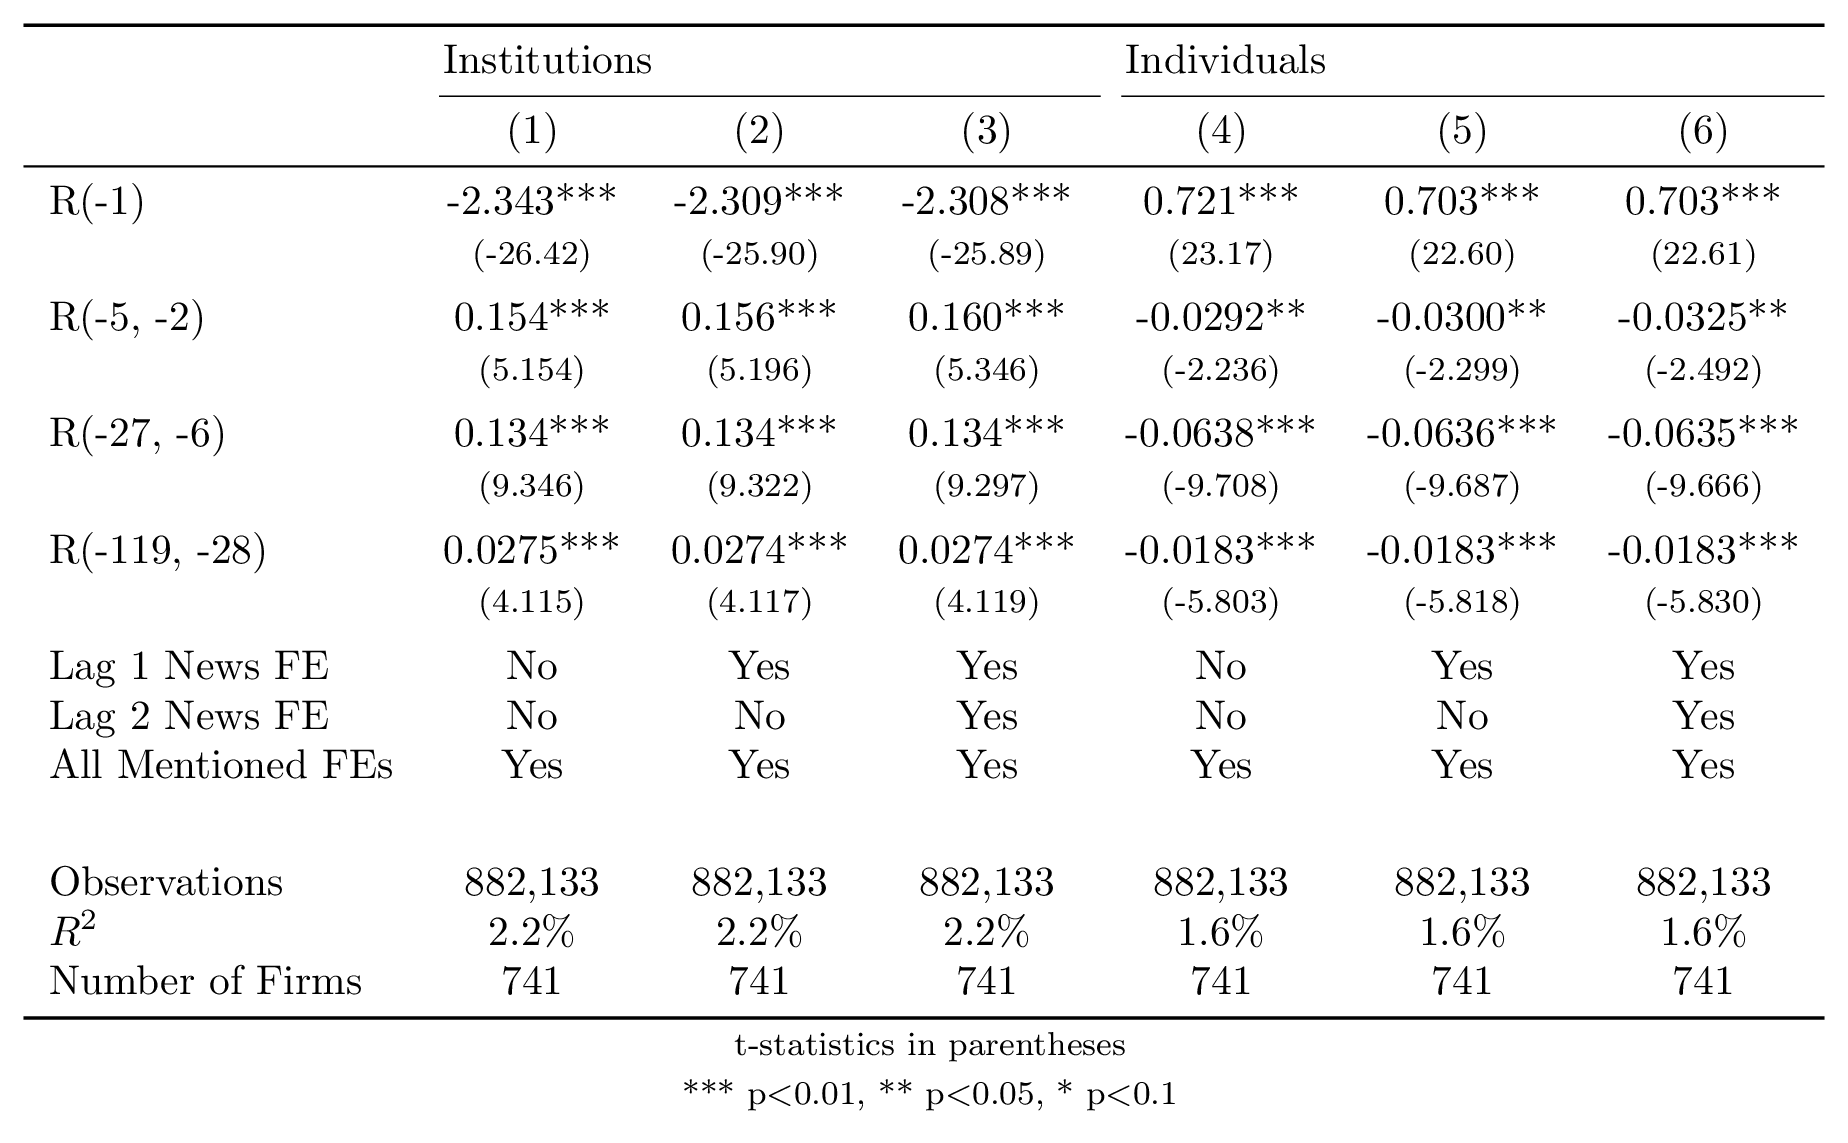
\includegraphics[width=\textwidth]{v5.png}
        \end{figure}
    \end{block}
\end{frame}


\subsection{Results by Firm Size}

\begin{frame}{Large VS. Small Firms}
    \begin{figure}
        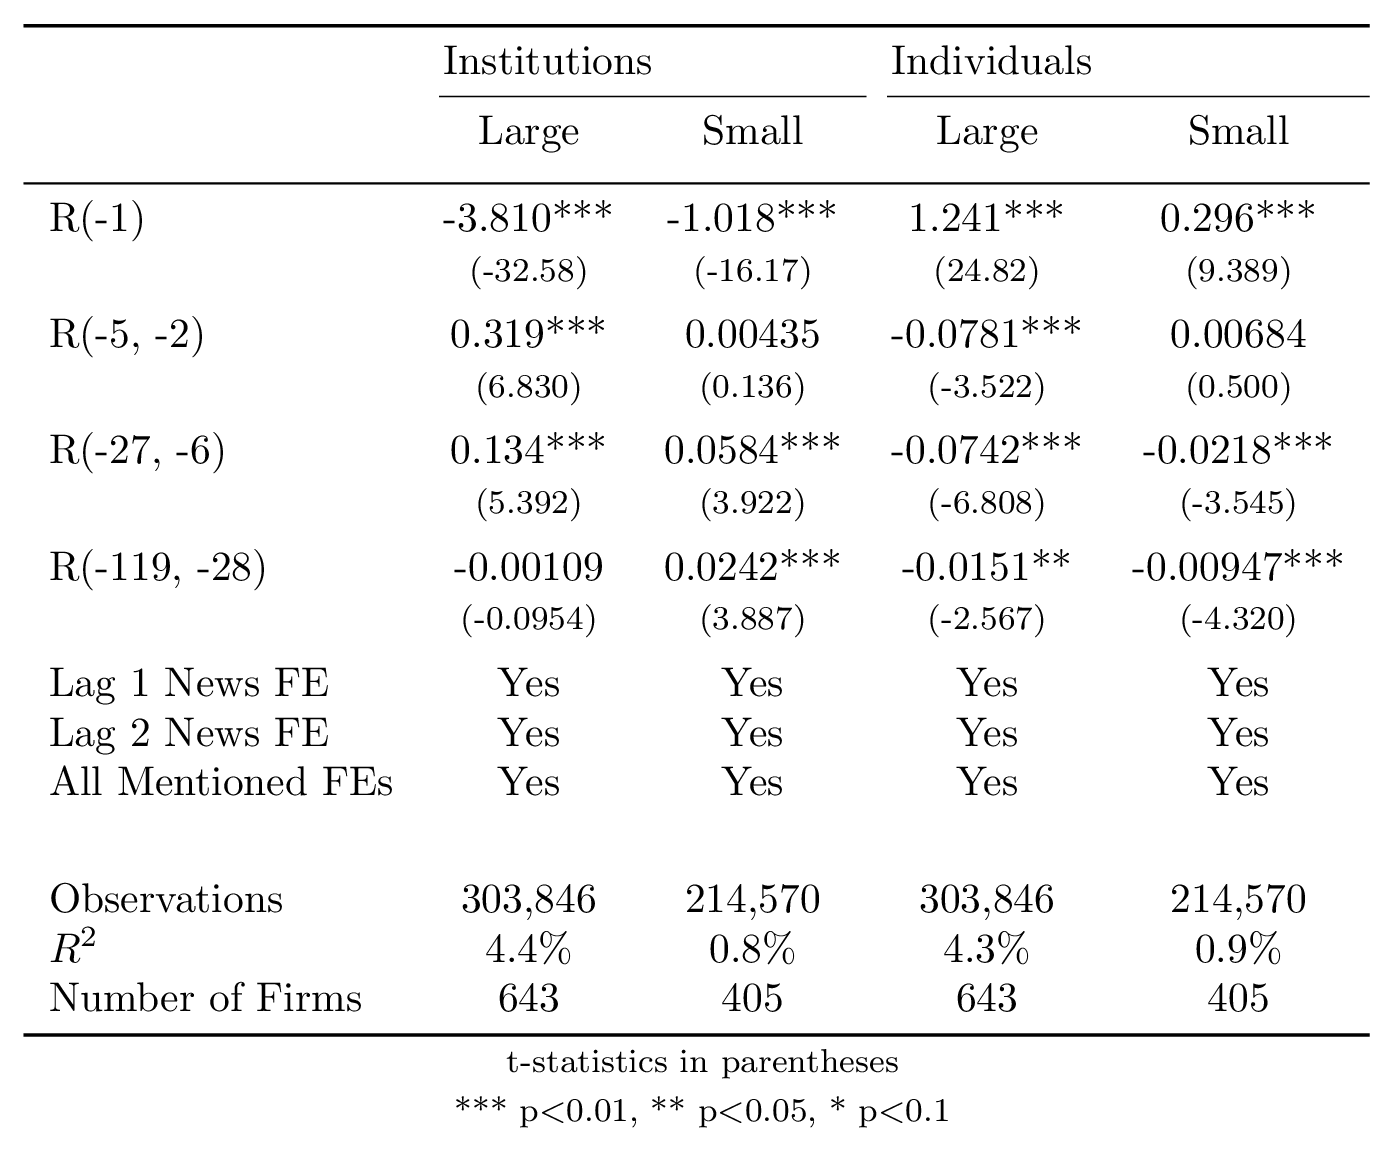
\includegraphics[scale = .2]{size.png}
    \end{figure}
\end{frame}


\section{Robustness Checks}
\subsection{Count Imbalance}

\begin{frame}{Count Imbalance Index}
    \begin{figure}
        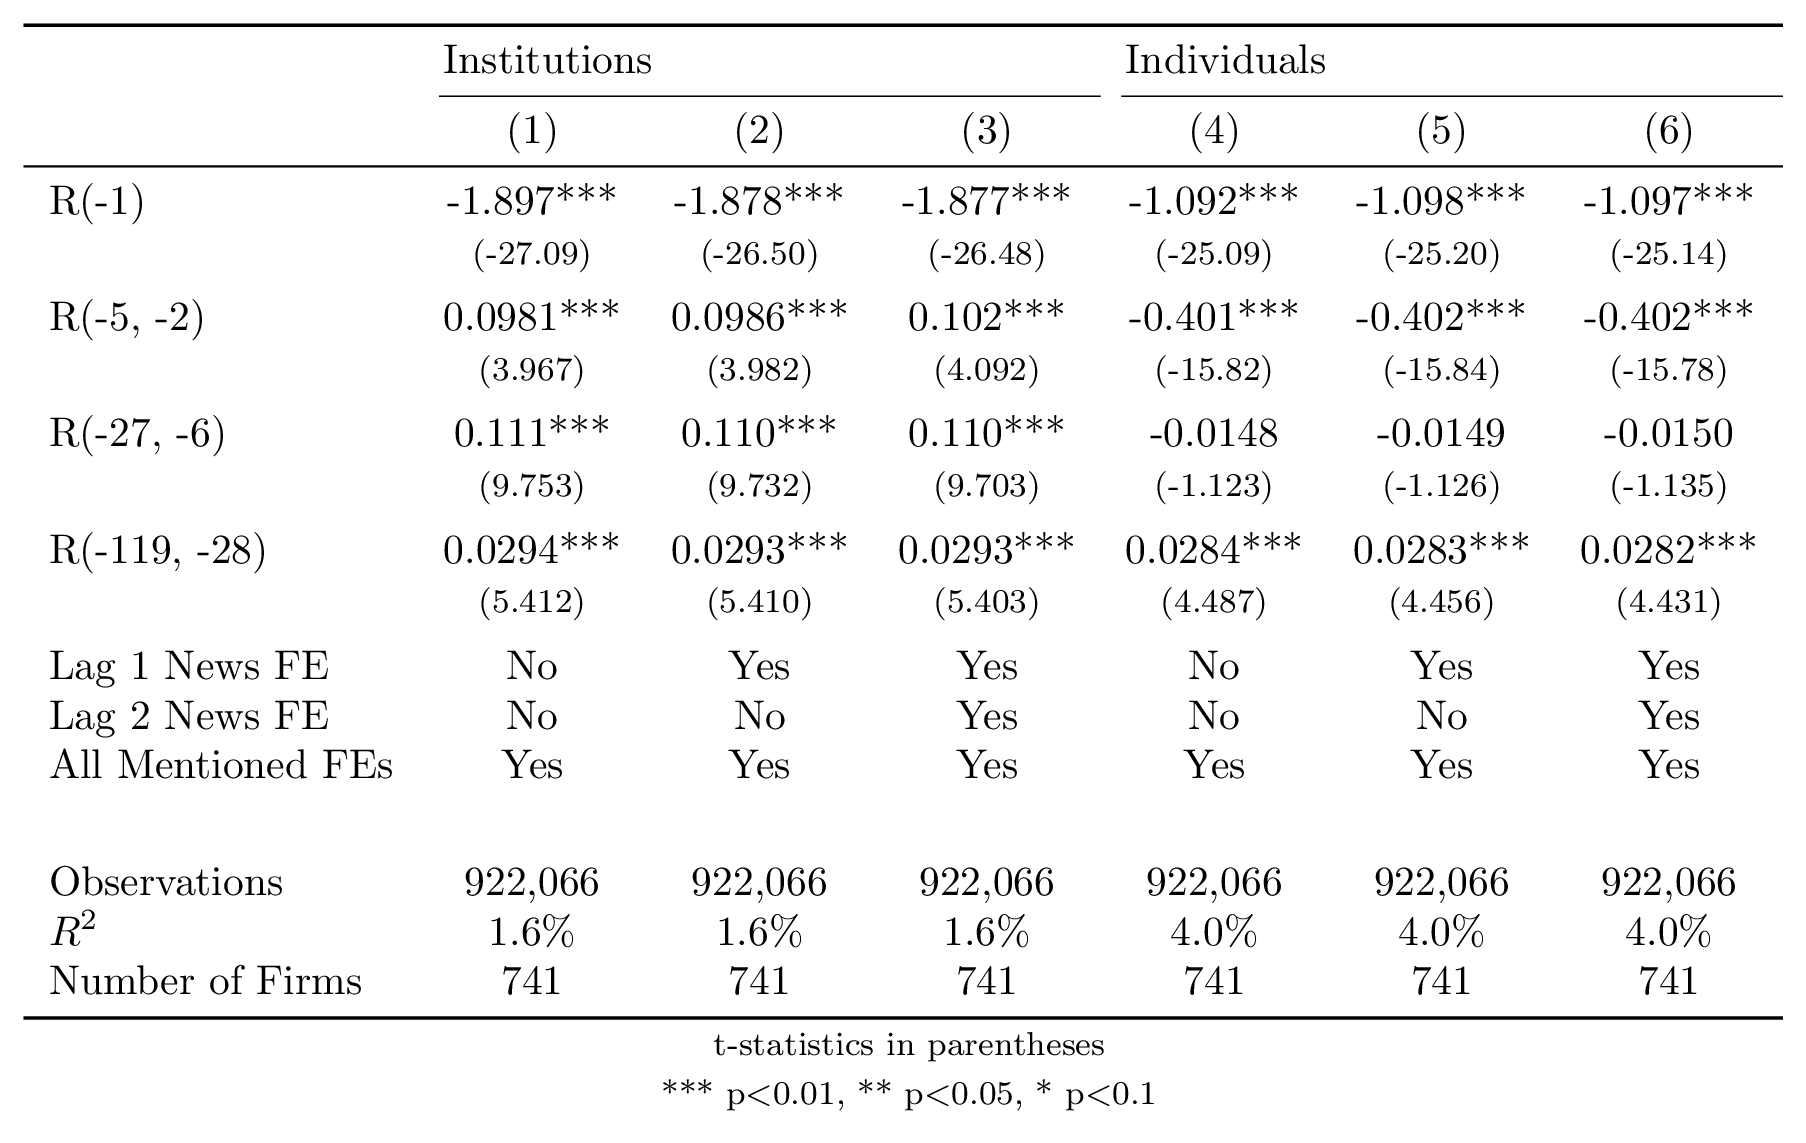
\includegraphics[width=\textwidth]{ci.png}
    \end{figure}
\end{frame}


\subsection{No News Days}


\begin{frame}{No News Days}
    \begin{figure}
        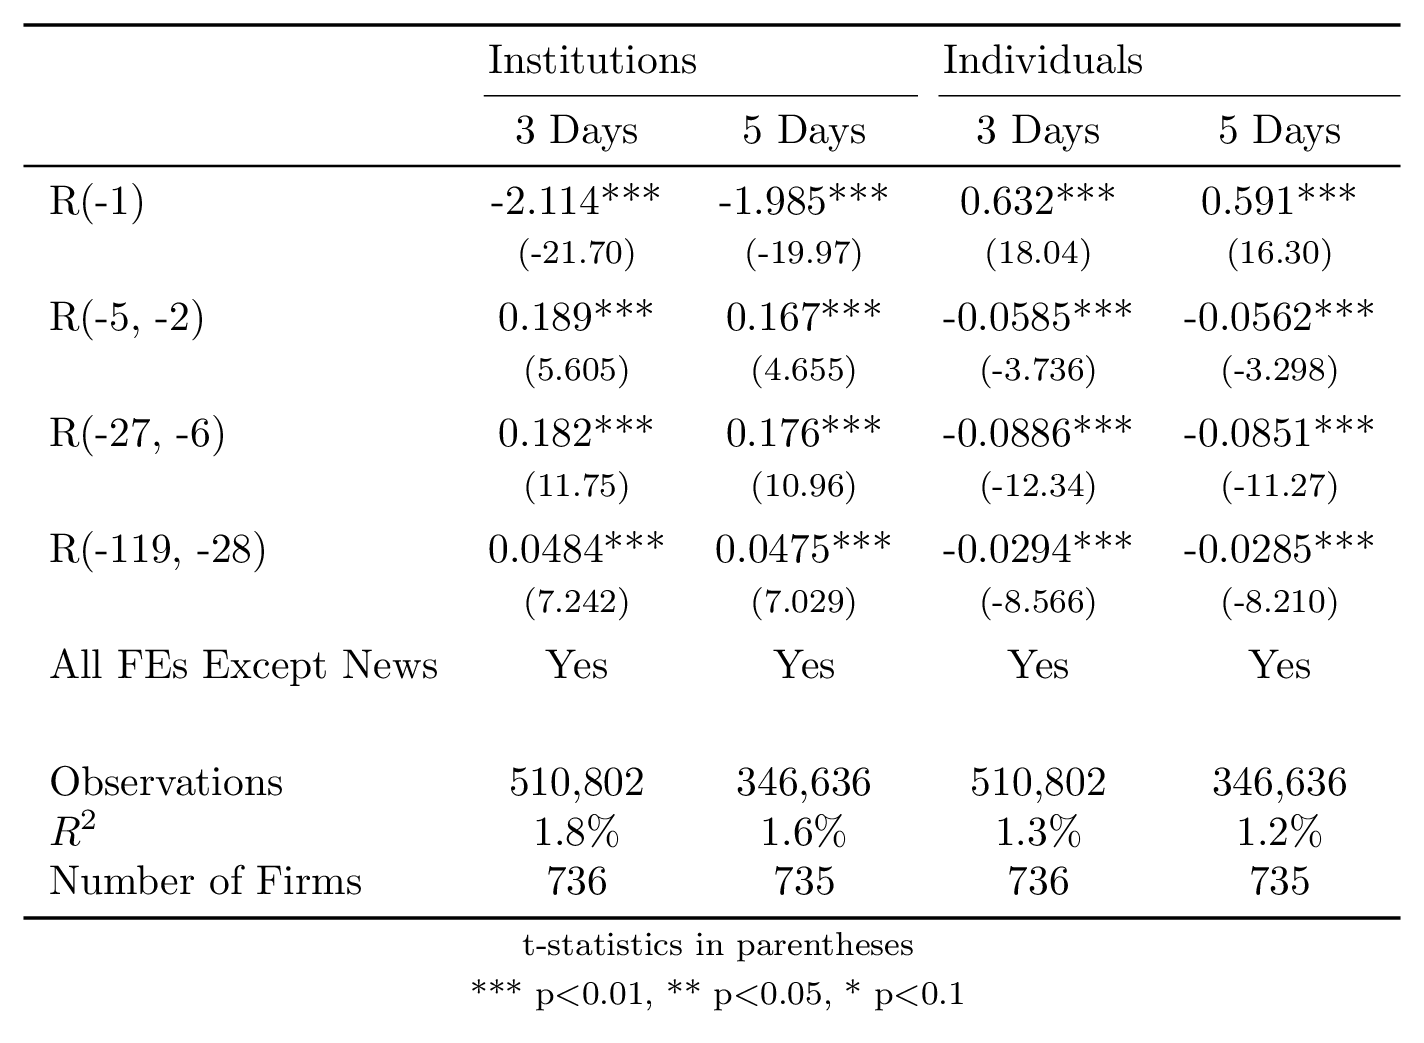
\includegraphics[scale = .22]{nonews.png}
    \end{figure}
\end{frame}


\section{Conculsion}


\begin{frame}{Conculsion}
    \begin{itemize}
        \item The present study introduces an approach to categorize stock-specific news into positive and negative classifications.
        \item The findings suggest that institutions tend to go against momentum trading in the context of a one-day holding period. Conversely, for the three longer time horizons, institutions seem to adopt a momentum-oriented strategy.
        \item On the other hand, the results reveal that individuals engage in momentum trading within a one-day holding period but shift towards an anti-momentum approach for longer horizons.
    \end{itemize}
\end{frame}











\end{document}